\section{使用者操作說明}
\label{sec:manual}

\subsection{按鍵說明}

場景沿用 Homework \#2 的機器人與地形世界。這次機器人與相機分開操作，兩者在任何模式下都不會互相影響（表~\ref{tab:controls}）。

\begin{table}[htbp]
    \centering
    \caption{按鍵說明}
    \label{tab:controls}
    \small
    \begin{minipage}[t]{.47\textwidth}
        \vspace{0pt}
        \centering
        \begin{tabular}{>{\bfseries}ll}
            \toprule
            \multicolumn{2}{l}{\textit{機器人}}  \\
            \midrule
            W / S        & 沿自己的朝向前進 / 後退      \\
            A / D        & 往左 / 右平移           \\
            Q / E        & 原地左轉 / 右轉          \\
            左 Shift      & 按住時跑步              \\
            空白鍵          & 跳躍                 \\
            1 / 2 / 3    & 站立 / 潛行 / 坐下       \\
            \midrule
            \multicolumn{2}{l}{\textit{投影方式}} \\
            \midrule
            F1 / F2 / F3 & 沿 x / y / z 軸平行投影  \\
            F4           & 透視投影（預設）           \\
            F5           & 四個 viewport        \\
            \bottomrule
        \end{tabular}
    \end{minipage}\hfill
    \begin{minipage}[t]{.5\textwidth}
        \vspace{0pt}
        \centering
        \begin{tabular}{>{\bfseries}ll}
            \toprule
            \multicolumn{2}{l}{\textit{相機}}               \\
            \midrule
            I / K                        & 前進 / 後退（surge） \\
            J / L                        & 往左 / 右平移（sway） \\
            U / O                        & 上升 / 下降（heave） \\
            $\leftarrow$ / $\rightarrow$ & 左轉 / 右轉（yaw）   \\
            $\uparrow$ / $\downarrow$    & 抬頭 / 低頭（pitch） \\
            , / .                        & 往左 / 右傾斜（roll） \\
            左鍵拖曳                         & 往拖曳的方向看        \\
            = / -                        & 放大 / 縮小        \\
            R                            & 回到機器人後方        \\
            Tab                          & 切換跟隨 / 自由      \\
            \bottomrule
        \end{tabular}
    \end{minipage}
\end{table}

\subsection{畫面}

左上角的 HUD 顯示目前的投影方式與相機模式、相機的 eye、focus、view up 與視角 fovY，
以及機器人的朝向、位置與速度，方便對照操作前後觀察參數的變化。
畫面分成多個 viewport 時，每一塊的左下角會標出它使用的投影方式（圖~\ref{fig:quad}）。

\begin{figure}[htbp]
    \centering
    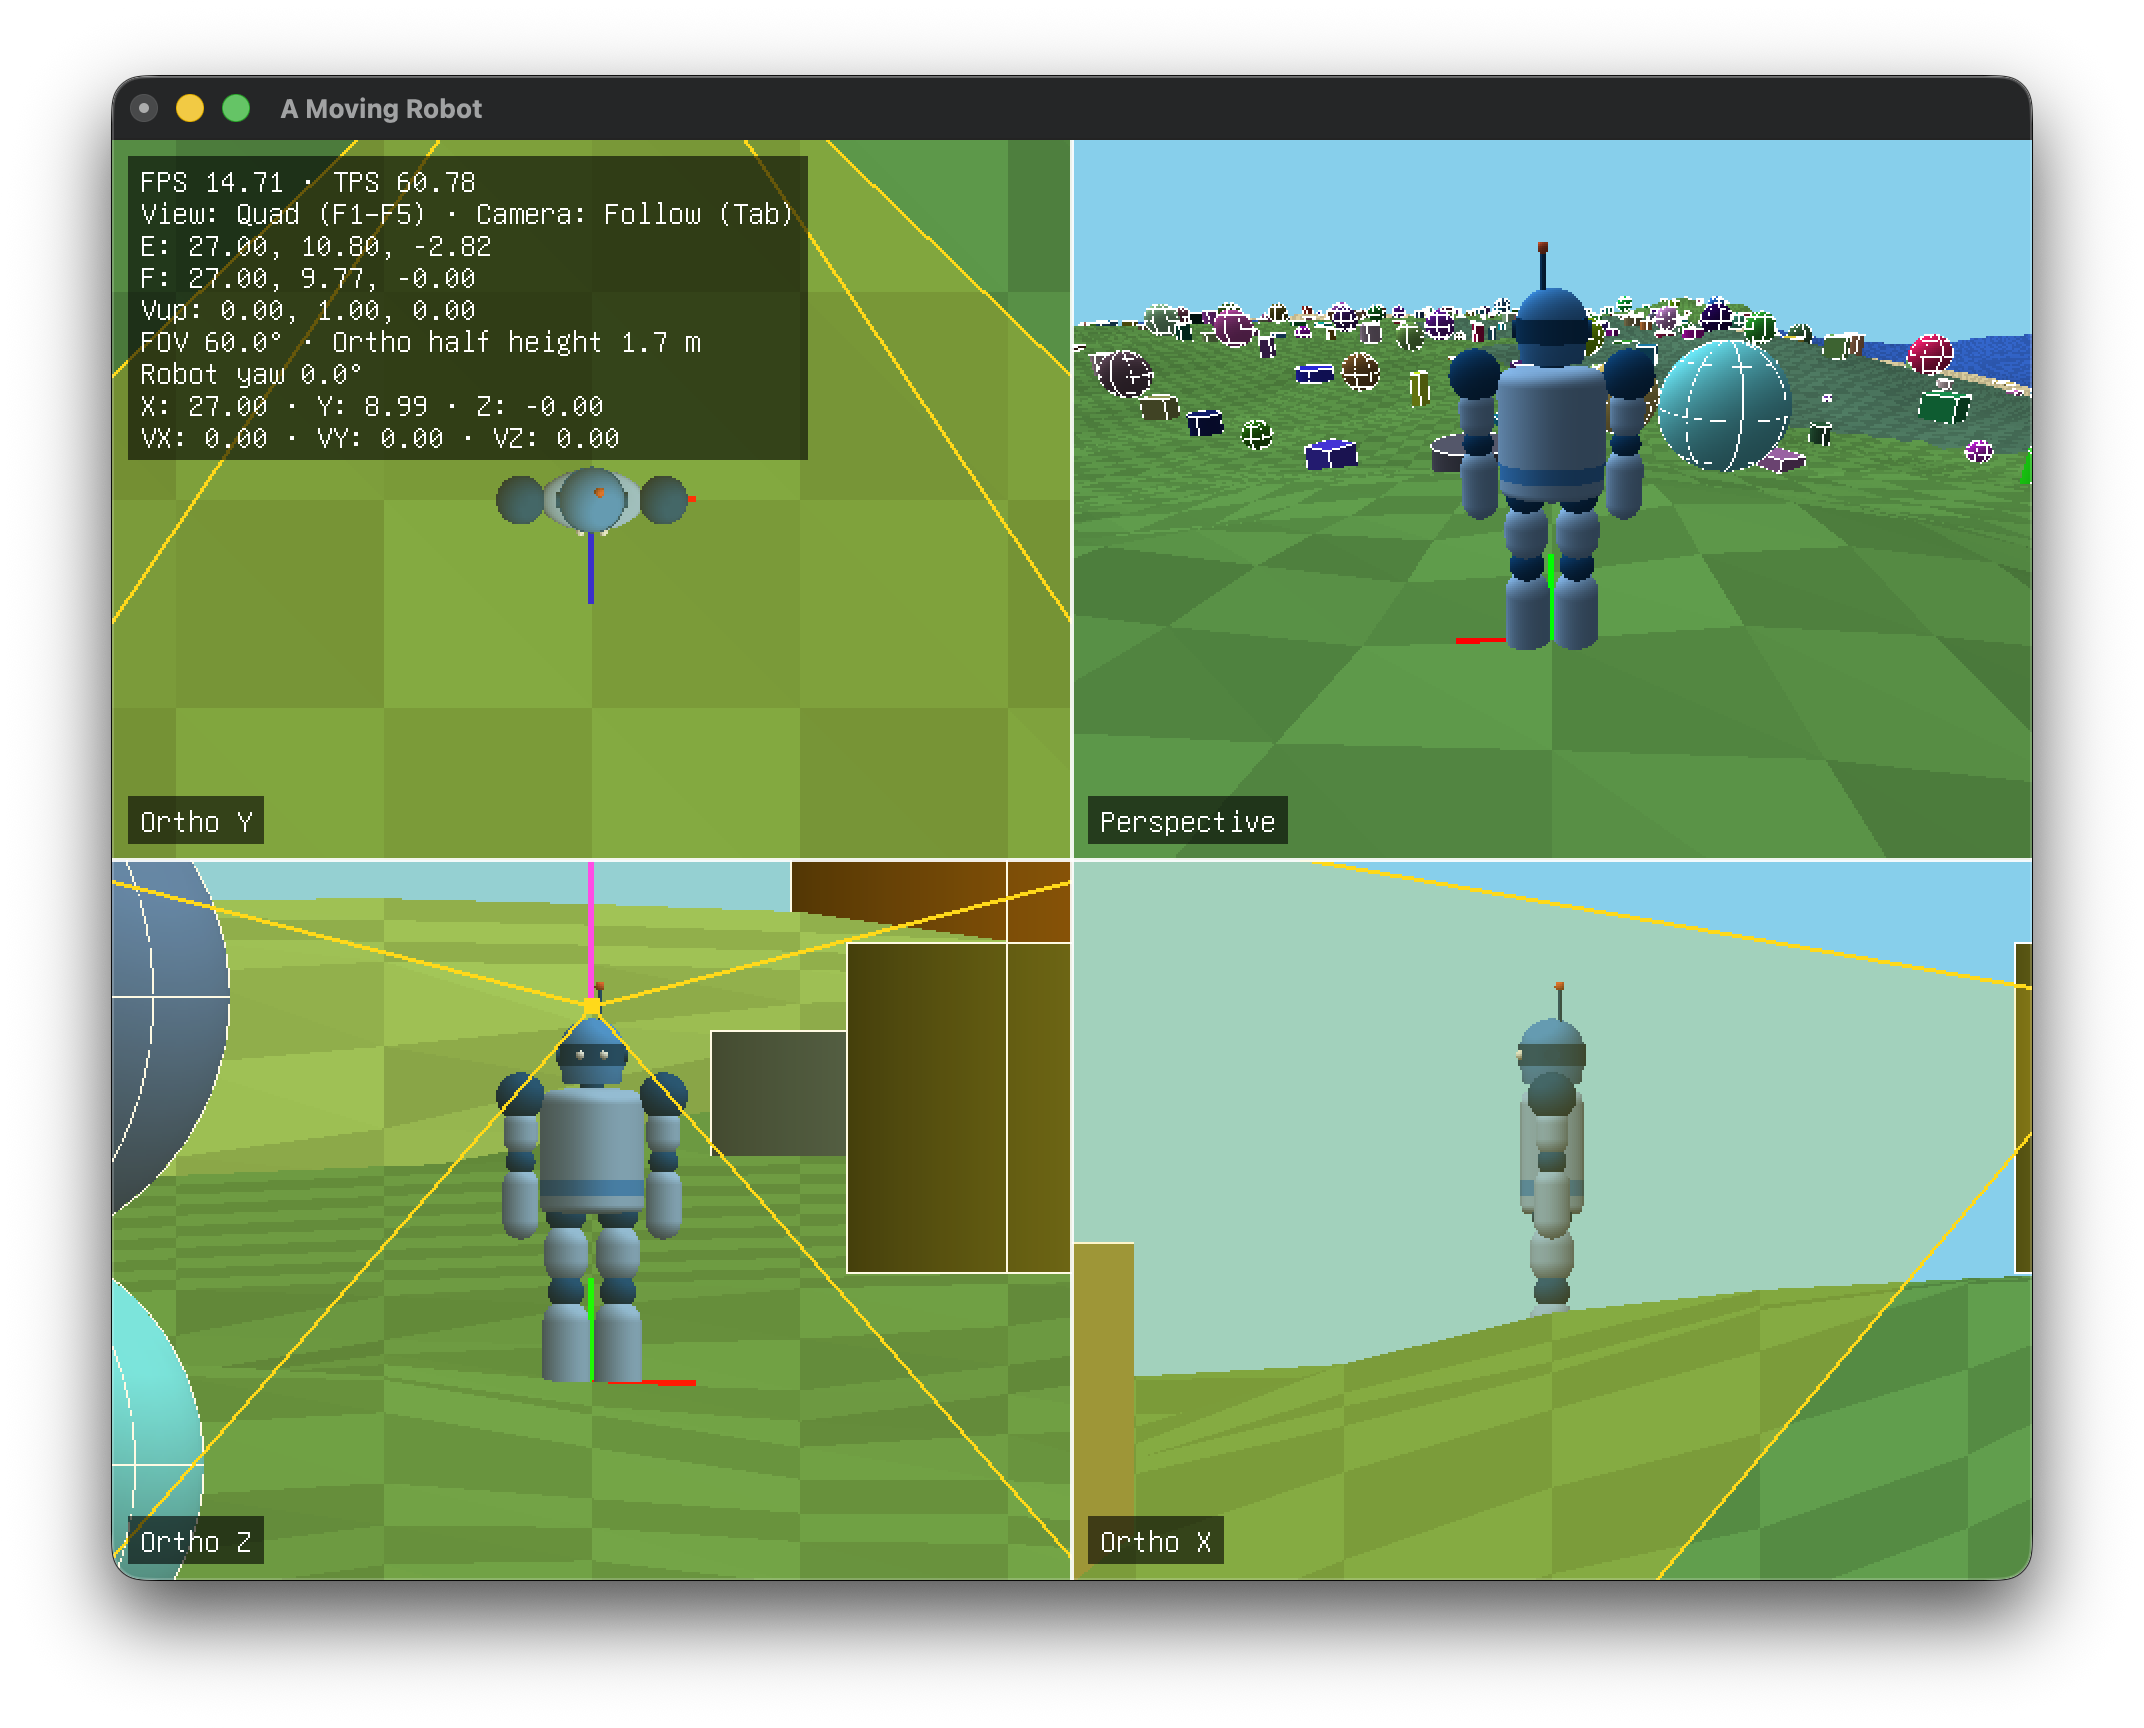
\includegraphics[width=.75\textwidth]{docs/figures/hw3/quad-view.png}
    \caption{四個 viewport：左上俯視、右上透視、左下前視、右下右側視}
    \label{fig:quad}
\end{figure}
